%!TEX root = ../main.tex
%
% ニュートンリング
%


\section{ニュートンリング}

\subsection{ニュートンリング実験器}

ニュートンリングとは、平凸レンズと平面のガラス板を組み合わせ、そこに光を当て
たときに入射光と反射光の干渉効果によって生じるリング状の光の縞模様のことです。
このリングのサイズを測定するための装置がニュートンリング実験器です。
この実験器は、次のような目的に使うことができます。

\begin{enumerate}

\item 波長の分かっている単色光源を用いてニュートンリングを作り、リングの大き
さを測定することによって、レンズの曲率半径を求める。

\item 曲率半径の分かっているレンズを用い、単色光源を当ててニュートンリングを
作り、リングの大きさを測定することによって、単色光源の波長を求める。

\end{enumerate}

\subsection{測定原理}

\begin{wrapfigure}[11]{r}{7cm}
\vspace*{-0.8cm}
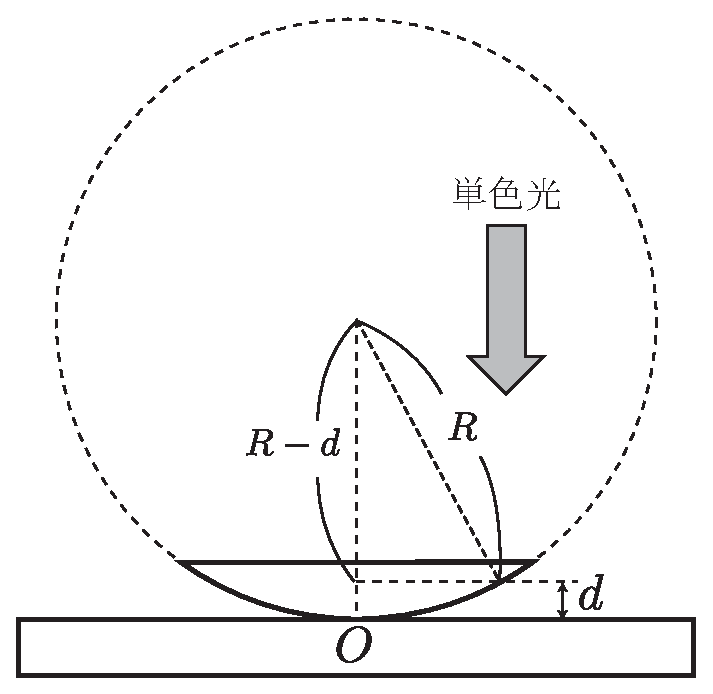
\includegraphics[scale=0.6]{04_Newton/newton.eps}
\end{wrapfigure}


右図のように、平面ガラス板の上に平凸レンズを置くと、凸レンズ面とガラス
板の間に薄い空気の層ができます。

このガラス板に垂直になるように、上面から光が入射したとき、平凸レンズの
下面で反射した光と、平面ガラス板の上面で反射した光が干渉し、干渉縞が生じ
ます 。

右図の点Aの位置に光が入射したときの、平凸レンズと平面ガラスの間の空気の層の厚さを$d$とします。
空気の層は非常に薄いので、入射光と反射光はほぼ平行とみなすことができるため、
入射光と反射光が通った道のりの差(光路差)は、$2d$と表わすことができます。

このことから、レンズの凸面の曲率半径を$R$とし、凸面とガラス面との接点Oから 
光の入射点までの距離を$r$とすると、次の関係式が成り立ちます。
\begin{eqnarray}
&&r^2 = R^2-(R-d)^2 = 2Rd-d^2\approx 2Rd\nonumber\\
&&\Rightarrow 2d=\frac{r^2}{R}\nonumber
\end{eqnarray}


平面ガラスの上面での光の反射は、空気からガラスへ向かう境界面での反射なので、
(ガラスの方が光学的に密であるため)固定端の反射となり、位相が反転します。その
ため、光路差が光の波長$\lambda$の整数倍のときは、入射光と反射光は逆位相で干渉して暗くな
ります。この時の$r$と$R$, $\lambda$との関係は次のようになります。
\begin{eqnarray}
&&\frac{r^2}{R}=m\lambda\nonumber\\
&&\Rightarrow r^2=m\lambda R
\qquad (m=0,1,2,3,\ldots)\nonumber
\end{eqnarray}
この条件を満たす位置を上方から見ると、点Oを中心とした暗い円が観測されることになります。

実際にはレンズの凸面とガラスの平面が正確に中心で接していないことから、そのず
れの大きさを$\delta$とおくと、光路差は$2(d+\delta)$となり、先ほどの暗い円が見られるための
条件式は、
\[
r^2 = m\lambda R-2\delta R
\]
となるので、中心から$m$番目の円の半径$r_m$と$m+n$番目の半径$r_{m+n}$を求めると、
このずれの大きさを消去してやることができます。
\[
\left\{
\begin{array}{l}
r_m^2=m\lambda R-2\delta R\\
r_{m+n}^2=(m+n)\lambda R-2\delta R
\end{array}
\right.
\] 
\begin{equation}
\Rightarrow
\boxed{
\lambda R =\frac{r_{m+n}^2 - r_m^2}{n}
}
\label{Newton}
\end{equation}
実際の測定ではこの式を用いて計算を行います。$\Rightarrow${\bf [実験 4-1]}


\newpage

\jikken

\begin{itemsquarebox}[c]{\bf 実験用具}
ニュートンリング実験器(マイクロメーターつき顕微鏡、ニュートンリング板 、
ハーフミラー)、ナトリウムランプ
\end{itemsquarebox}

\bigskip

\subjikken{ニュートンリング実験器による単色光の波長の測定}


ニュートンリング実験器は、マイクロメーターつきの
移動顕微鏡、ハーフミラー、ニュートンリング板(平
凸レンズと平面ガラスを合わせたもの)をセットした
レンズ容器の支持台で構成されています。顕微鏡の倍
率は約10倍で、マイクロメーターで左右に移動する
ことができます。

\begin{enumerate}

\item 平凸レンズの凸面を下にして平面ガラスの上に重
ね、レンズ容器に入れてレンズ支持台に固定してお
きます。(通常は最初からセットしてあります。)

\item ナトリウムランプを点灯し、その光を$45^\circ$に傾け
たハーフミラーに入射させてガラス板に当てます。
光が当たると、肉眼でもレンズの中心付近に小さな
ニュートンリングが見えます。

\item 最初に顕微鏡の接眼部を回して顕微鏡の視野の十字線のピントを合わせます。
十字線がはっきり見えたら、これ以降接眼部はさわらないようにします。

\item マイクロメーターの目盛りは0〜25 [mm] なので、最初は目盛りの中心辺りの
12 [mm]付近に目盛りを合わせ、このとき十字線の中心にニュートンリングの中心
が来るように、レンズ容器の位置を調節してやります。

\item 測定は、誤差を少なくするため、暗円の直径を測定して半径を算出する方法を用
います。中心の黒丸を0番目とし、次の暗線を1番目として数えていき、5番目
以降の輪の直径を測定し、10番目の輪の直径まで、以下に述べるような順序で測
定を行ないます。また、マイクロメーターは逆回転させる際に誤差が生じやすい
ため、測定中は必ず一方方向にだけ、つまみを回していくようにします。

\begin{enumerate}

\item まず10番目の輪の左側の線に十字線の中心を合わせて、その時のマイク 
ロメーターの値:$a_{10}$を読み取り、記録します。(10番目の輪が見えない 
場合は、測定可能な輪のうち一番外側の輪の左側に合わせます。)

\item マイクロメーターを動かして十字線の中心を少しずつ右にずらし、9番目 
の輪、8番目の輪の左側の線の場所、$a_9$, $a_8$を同様にして測定していき 
ます。

\item 5番目の輪の位置($a_5$)まで記録したら、今度は5番目の輪の右側の線
まで十字線の中心を移動し、この場所:$a_5'$を記録します。同様にして、
10番目の輪の右側の位置:$a_{10}'$まで、順番に測定します。(なるべく外側
の輪のデータを用いた方が正確に測定できるので、見えていれば15番
目の輪の位置まで測定しましょう。)

\item 輪の直径と半径を求めていきます。
\[
2r_5= a_5'-a_5 \quad \Rightarrow \quad r_5=\frac{a_5'-a_5}{2}
\]
のようにして、 $r_5\sim r_{10}$まで、それぞれ半径を求めます。

\item ニュートンリング板の曲率半径を2000 [mm]とし、(\ref{Newton})式を用い
てナトリウムランプの波長λを求めます。$n=3$とし、$m=5, 6, 7$の3通
りについて$\lambda$を計算し、それらの値の平均値を求めましょう。


\end{enumerate}


\end{enumerate}



\hspace*{-\parindent}
※ ナトリウムランプの波長を理科年表で調べ、自分達の測定結果と比較しましょう。

